\section{System Architecture}
\label{sec:architecture}

At its most basic, the OPQ system architecture is extremely simple: OPQ Boxes are plugged into wall outlets, they monitor the quality of power at their wall outlets, and the results are communicated via the Internet to a software system called OPQ Cloud. To see the results, users login to the system using a browser.

A slightly less basic description is this: the OPQ system architecture consists of four major open source hardware and software components that provide end-to-end support for the capture, triggering, analysis, and reporting of consumer level local and global PQ events.

\begin{enumerate}

\item OPQ Box is a hardware device that detects the electrical waveform from a standard residential outlet and communicates both low and high fidelity representations of the waveform to other OPQ system components.

\item OPQ Makai monitors incoming low fidelity data from OPQ Boxes, requests high fidelity data when necessary, and stores the results in a MongoDB database.

\item OPQ Mauka analyzes data, creates "events" when it detects anomolies, and can tell OPQ Makai to request high fidelity data from one or more OPQ Boxes to facilitate analysis.

\item OPQ View is a visualization platform for displaying the results for data capture and analysis.

\end{enumerate}

\begin{figure}
\center 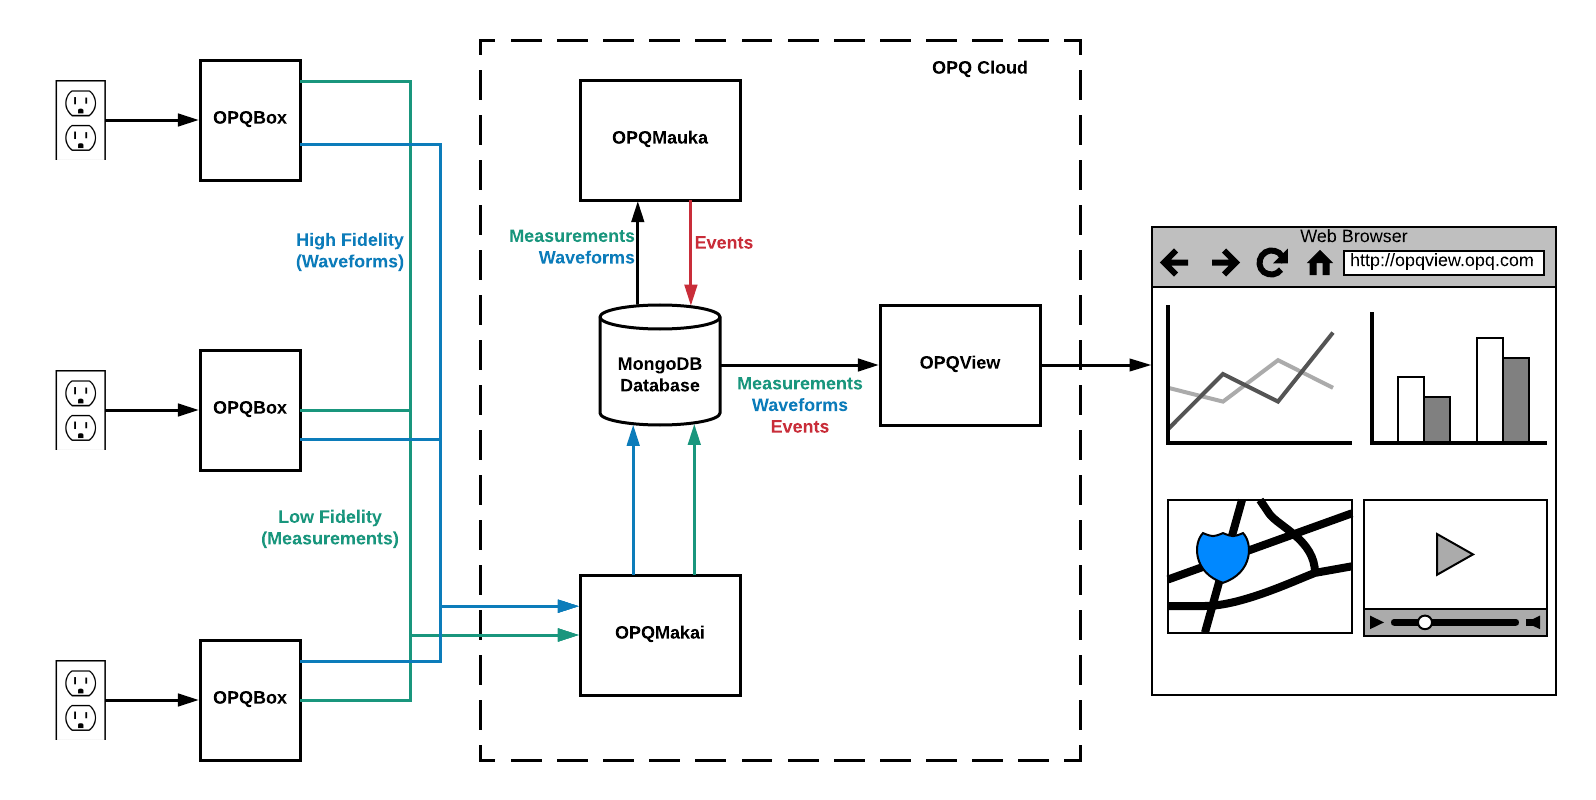
\includegraphics[width=5in]{images/system-diagram.png}
\caption{High level architecture of the OPQ System}
\label{fig:architecture}
\end{figure}


Figure \ref{fig:architecture} illustrates how these components work together to take information from wall outlets (on the left side) to the display of analyses in a browser (on the right hand side).  First, OPQ Boxes analyze power from wall outlets, and send low fidelity measurements to OPQMakai. OPQ Makai analyzes low fidelity measurements, and requests high fidelity waveforms when desirable. Both measurements and waveforms are saved in a MongoDB database. OPQ Mauka analyzes low and high fidelity data, and creates "events" to represent anomalies. OPQ View notifies users of events and allows them to drill down into low and high fidelity data.

OPQ Makai, OPQ Mauka, and OPQ View are all cloud-based software services that collectively form a single "instance" with respect to data transmission, storage, analysis, and visualization. We refer to this collection of software-side components as OPQ Cloud. Every OPQ Box connects to a single instance of an OPQ Cloud. It is possible to have multiple OPQ Cloud instances. For example, a company might install an OPQ Cloud instance behind their firewall along with OPQ Boxes to provide a private mechanism for collecting and analyzing power quality data.

This architecture has a number of benefits. The combination of low and high fidelity data reduces both network overhead and storage requirements, which increases the scalability of the system in terms of the number of OPQ Boxes that can be tied to a single OPQ Cloud instance. OPQ Makai and OPQ Mauka have a plugin architecture, making it easier to extend their functionality to incorporate new triggers for high quality data (in the case of OPQ Makai) and new events and analyses (in the case of OPQ Mauka). Finally, the open source licensing of both hardware and software makes it possible to incorporate new ideas, bug fixes, and enhancements from technologists across the power quality community.

\section{Information Architecture}

OPQ's "information architecture" is designed to facilitate the process of generating actionable, useful insights into the nature of the electrical grid starting with the data collected from a wall outlet. It is a five layer architecture in which data in the form of Measurements collected by an OPQ Box can eventually yield insights in the form of Phenomena. (The Incident and Phenomena levels are currently in development.)

Table \ref{fig:information-architecture} provides an overview of the five layers from lowest level (Box) to highest level (Phenomena). "TTL", to Time To Live, indicates how long entities at each level are stored before they are automatically deleted.

\begin{table}[H]
\caption{OPQ Information Architecture Levels}
\centering
%% \tablesize{} %% You can specify the fontsize here, e.g., \tablesize{\footnotesize}. If commented out \small will be used.
\begin{tabular}{llp{4in}}
\toprule
\textbf{Layer}	& \textbf{TTL}	& \textbf{Purpose}\\
\midrule
Box		& 1 hour			& Collects and holds a rolling one hour window of "high fidelity" wave form data for a single location.\\
Measurement		& 1 day			& Approximately once a second, each box sends a Measurement to OPQ Cloud. Measurements provides "low fidelity" summary statistics regarding four power measurements (Frequency, Voltage, THD, Transients). Measurements give OPQ Cloud basic situational awareness of the grid without the overhead of transmitting and storing wave form data. Measurements exist for one day, though a daily roll-up of Measurement summary statistics called "Trends" persists much longer.\\
Event & 1 month & When OPQ Cloud's Makai service detects non-nominal values in the stream of Measurements, it can decide to request wave form data from one or more boxes for a specific time interval (typically just a second or so). Note that Makai only has one hour to request high fidelity wave form data before it is written over in the Box.\\
Incident & 6 months & Not every non-nominal power data value is significant, i.e. actually meaningful for gaining insight into the grid. Over the years, electrical engineers have developed a variety of standards (IEEE 1159, ITIC, SEMA, etc.) for characterizing significant power quality events. OPQ Cloud's Mauka service provides classification algorithms to analyze each Event to see if it satisfies any of the standards for significance. If so, an Incident is created, indicating that a significant PQ event has occurred at a specific time in a specific location. Each Incident can also be annotated with context, which is additional information about the environment or other physical factors present at the time and location of this incident. Context can be manually provided by users or automatically associated with Incidents through APIs to online services.\\
Phenomena & 1 year & All of the prior levels represent behaviors of a individual Boxes in a single location at a given point in time. This final level of OPQ's information architecture is premised on the idea that insightful, actionable information results from the ability to either explain or else predict multiple Incidents. First, a Phenomena can be created in order to collect data from multiple Incidents with a common cause. An example of this form of phenomena is "the voltage drop experienced by all boxes in Kailua on 5/22/18 at 1:03pm was caused by a transformer trip at the Kailua substation." Second, a Phenomena can collect data from multiple Incidents in order to predict future Incidents. For example, "when winds exceed 40 knots in Kahuku, data from prior Incidents leads to the prediction that there will be a voltage surge of approximately 5V for approximately 3 seconds in all boxes located within 1 mile of Kahuku."\\
\bottomrule
\end{tabular}
\label{fig:information-architecture}
\end{table}




